Druhým zkoušeným způsobem vícevláknového vícevláknového výpočtu problému \textit{MBP} byl \textit{data paralelismus} opět pomocí knihovny \textit{OpenMP}.
Data paralelismus byl řešen následovně.
Nejprve se pomocí algoritmu \textit{BFS} získalo \textit{n} disjunktních stavů.
Tyto stavy byly následně předávány jednotlivým vláknům k dopočítání.
Pro předávání stavů byl využit konstrukt \verb|omp parallel for|, 
který dynamicky přiděloval vláknům úlohy.
Jako optimální \textit{n} se ukázala hodnota 150.

Opět bylo třeba zajistit exkluzivní přístup do proměnné přepisující maximální dosaženou hodnotu vah.
To bylo zajištěno opět pomocí \verb|omp critial|.

Oproti task paralelizaci došlo ke zlepšení.
Na 20 jádrech je úloha cca 3 krát rychlejší oproti sekvenčnímu.
Z grafu lze opět vyčíst, že s vyšším počtem jader se od 8 vlákna příliš nezvětšuje rychlost výpočtu.

\FloatBarrier
\begin{table}[]
    \begin{tabular}{l|rrr}
                    instance &    čas výpočtu &  počet vláken &  počet procesů \\
    \hline
    graf\_15\_8.txt & 134.350 &           2 &         1 \\
    graf\_15\_8.txt &  81.274 &           4 &         1 \\
    graf\_15\_8.txt &  47.339 &           8 &         1 \\
    graf\_15\_8.txt &  46.298 &          16 &         1 \\
    graf\_15\_8.txt &  40.918 &          20 &         1 \\
    graf\_18\_7.txt & 260.309 &           2 &         1 \\
    graf\_18\_7.txt & 153.900 &           4 &         1 \\
    graf\_18\_7.txt &  89.133 &           8 &         1 \\
    graf\_18\_7.txt &  78.588 &          16 &         1 \\
    graf\_18\_7.txt &  80.974 &          20 &         1 \\
    graf\_21\_6.txt & 177.718 &           2 &         1 \\
    graf\_21\_6.txt & 105.388 &           4 &         1 \\
    graf\_21\_6.txt &  60.699 &           8 &         1 \\
    graf\_21\_6.txt &  54.057 &          16 &         1 \\
    graf\_21\_6.txt &  52.689 &          20 &         1 \\
    \end{tabular}
\end{table}


\begin{figure}[!htbp]
\centerline{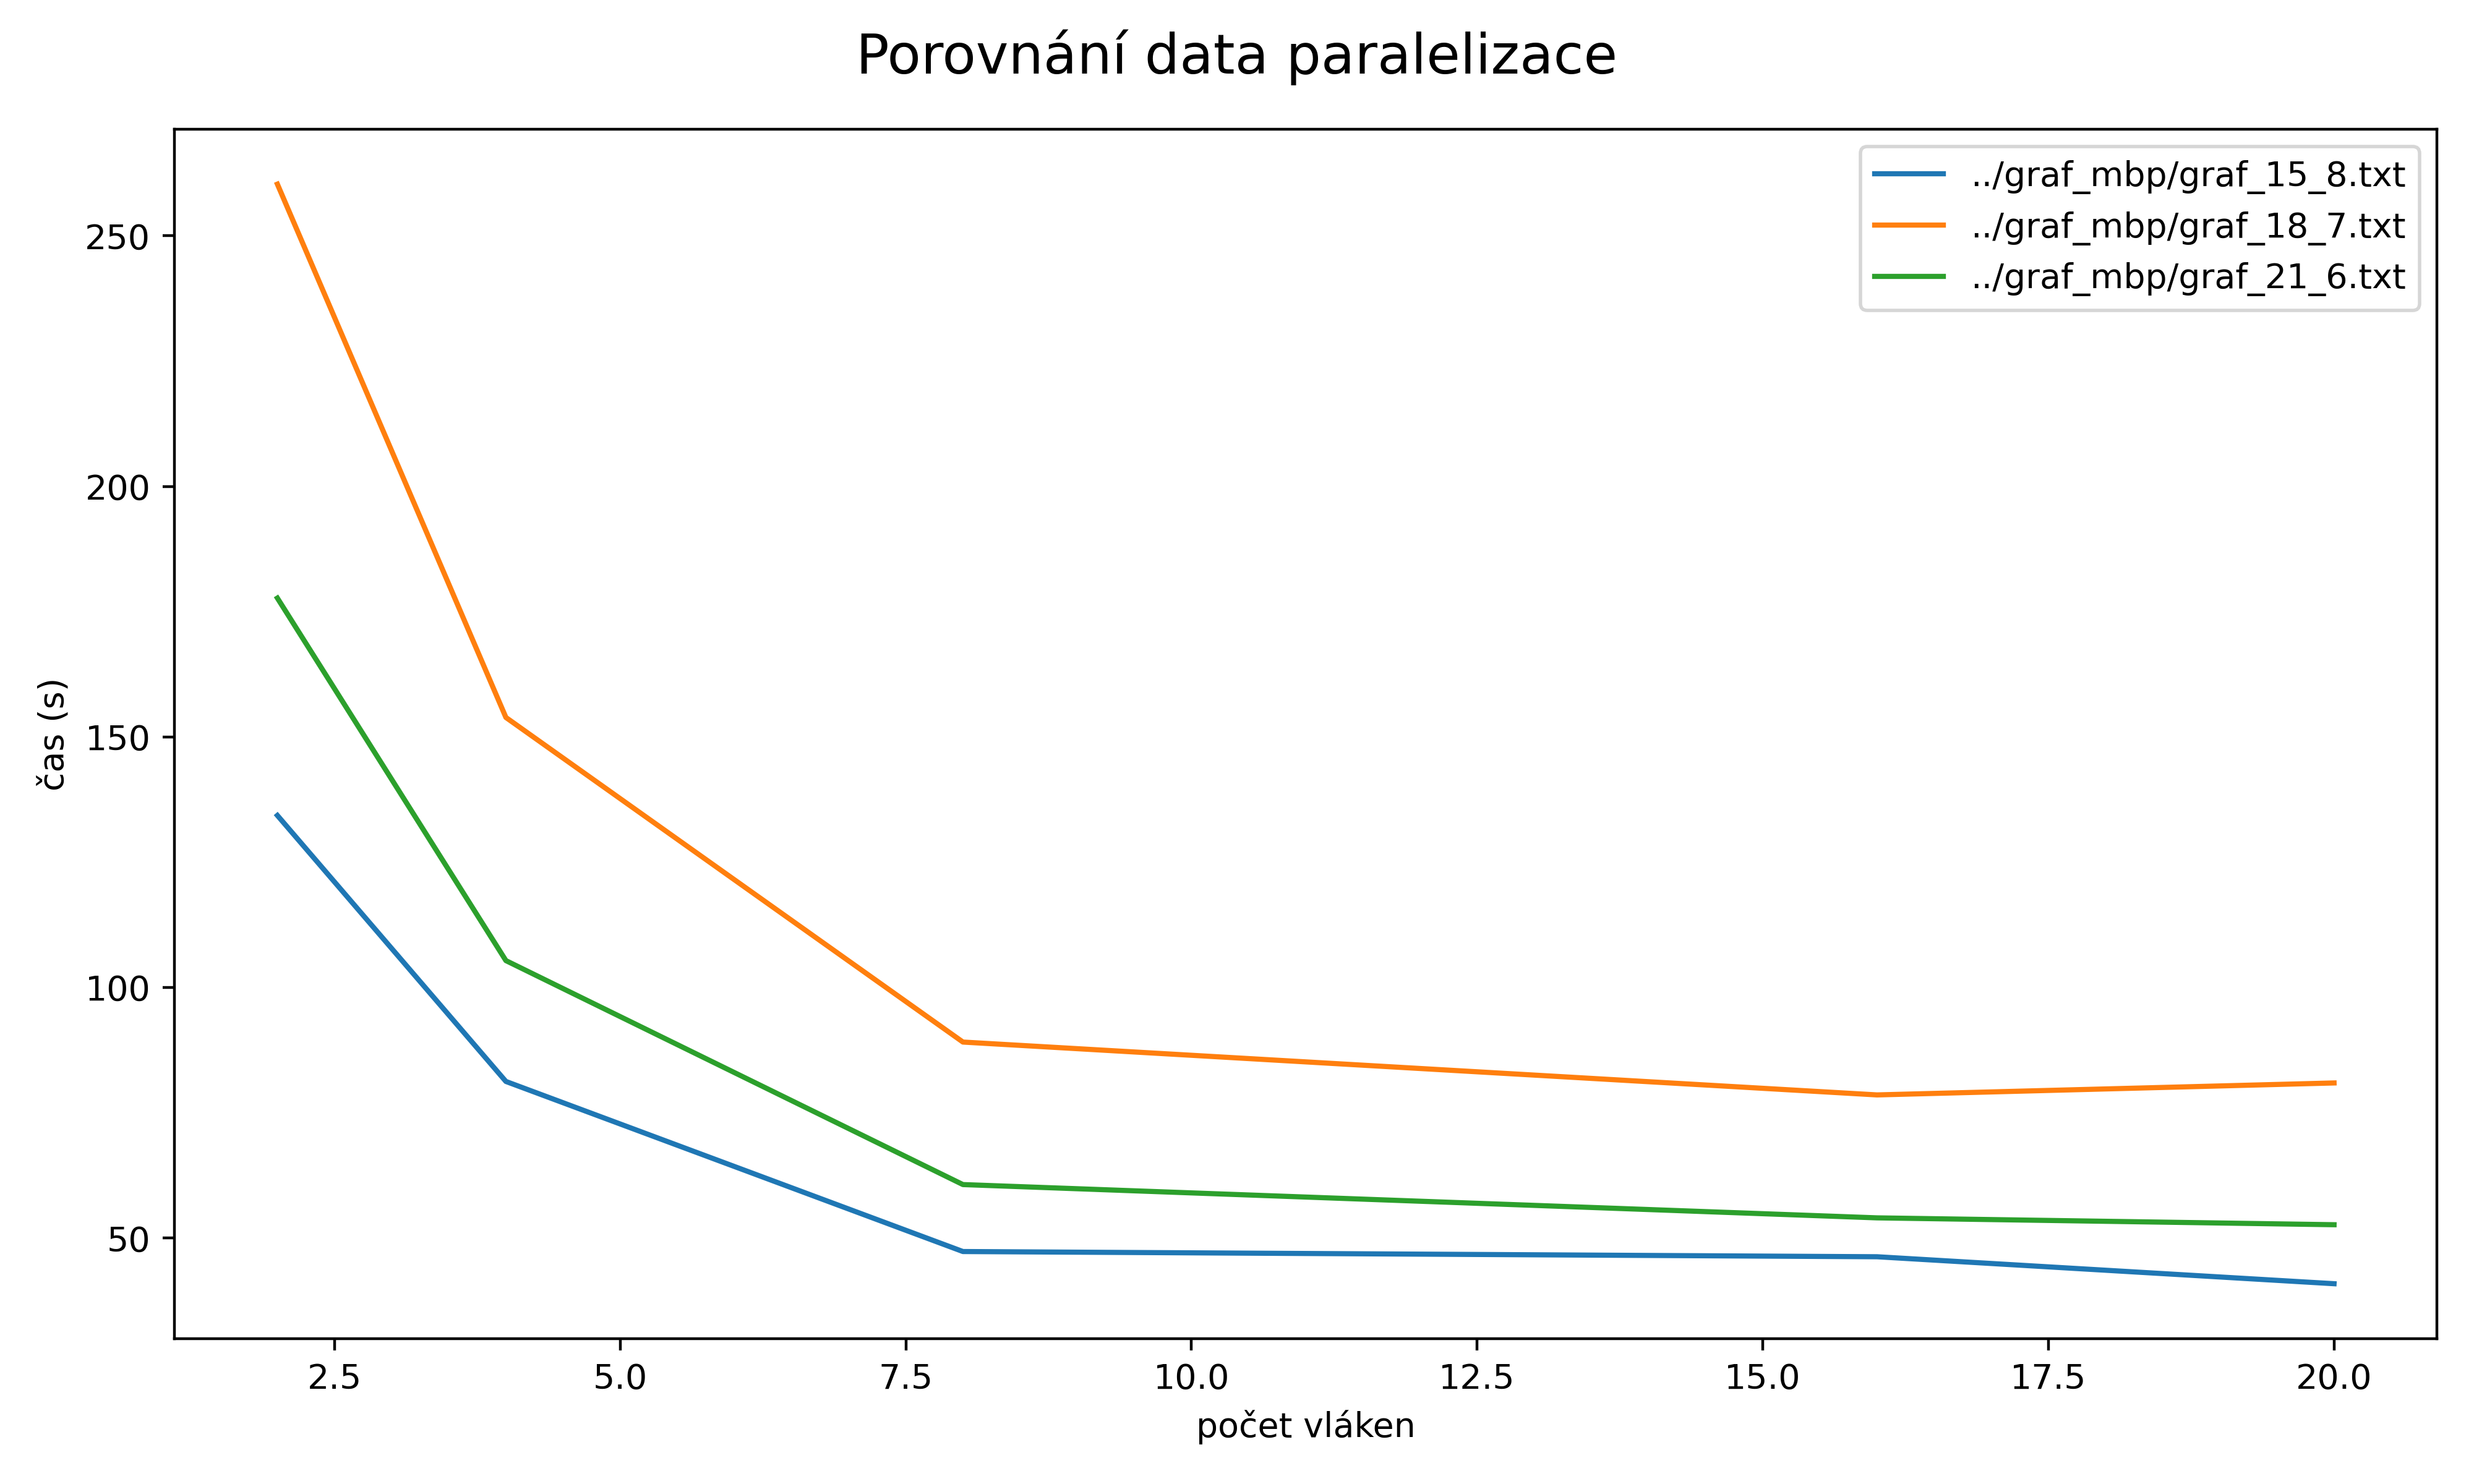
\includegraphics[scale=.46]{images/porovnání_data_paralelizace.png}}
\caption{Škálování OpenMP datové paralelizace}
\end{figure}
\FloatBarrier